\documentclass[10pt]{extarticle}
\title{}
\author{Avinash Iyer}
\date{}
\usepackage[shortlabels]{enumitem}

%font setup
%
%\usepackage{newpxtext,eulerpx}

%paper setup
\usepackage{geometry}
\geometry{letterpaper, portrait, margin=1in}
\usepackage{fancyhdr}

%symbols
\usepackage{amsmath}
\usepackage{amsfonts}
\usepackage{mathtools}
\usepackage{hyperref}
\usepackage{gensymb}

\usepackage[T1]{fontenc}
\usepackage[utf8]{inputenc}

\usepackage[version=4]{mhchem}
\usepackage{chemfig}

%plotting
\usepackage{pgfplots}
\usepackage{tikz}
\tikzset{middleweight/.style={pos = 0.5, fill=white}}
\tikzset{weight/.style={pos = 0.5, fill = white}}
\tikzset{lateweight/.style={pos = 0.75, fill = white}}
\tikzset{earlyweight/.style={pos = 0.25, fill=white}}

%\usepackage{natbib}

%graphics stuff
\usepackage{graphicx}
\graphicspath{ {./images/} }

%code stuff
%when using minted, make sure to add the -shell-escape flag
%you can use lstlisting if you don't want to use minted
%\usepackage{minted}
%\usemintedstyle{pastie}
%\newminted[javacode]{java}{frame=lines,framesep=2mm,linenos=true,fontsize=\footnotesize,tabsize=3,autogobble,}
%\newminted[cppcode]{cpp}{frame=lines,framesep=2mm,linenos=true,fontsize=\footnotesize,tabsize=3,autogobble,}

\usepackage{listings}
\usepackage{color}
\definecolor{dkgreen}{rgb}{0,0.6,0}
\definecolor{gray}{rgb}{0.5,0.5,0.5}
\definecolor{mauve}{rgb}{0.58,0,0.82}

\lstset{frame=tb,
	language=Java,
	aboveskip=3mm,
	belowskip=3mm,
	showstringspaces=false,
	columns=flexible,
	basicstyle={\small\ttfamily},
	numbers=none,
	numberstyle=\tiny\color{gray},
	keywordstyle=\color{blue},
	commentstyle=\color{dkgreen},
	stringstyle=\color{mauve},
	breaklines=true,
	breakatwhitespace=true,
	tabsize=3
}
% text + color boxes
\usepackage[most]{tcolorbox}
\tcbuselibrary{breakable}
\newtcolorbox{problem}[1]{colback = white, title = {#1}, breakable}
\newtcolorbox{solution}{colback = white, colframe = black!75!white, title = Solution, breakable}
%including PDFs
\usepackage{pdfpages}
\setlength{\parindent}{0pt}

\pagestyle{fancy}
\fancyhf{}
\rhead{Avinash Iyer}
\lhead{Econ 308: Class Notes}
\begin{document}
  \begin{problem}{Introduction to Public Economics}
    Governments play a crucial role in much economic life.
    \begin{itemize}
      \item Regulatory structure (financial markets, pharmaceuticals, labor markets, civil rights).
      \item Taxes.
      \item Public goods and social welfare spending.
      \item Macroeconomic stabilization.
    \end{itemize}
   Public finance is the study of the role of government in a market economy, primarily focusing on taxes and spending.\\

   Reasons to study public economics:
    \begin{itemize}
      \item Governments have a lot of power in the realm of economic welfare.
      \item Nearly every economic transition is mediated by the government.
      \item It can inform debates about the appropriate role of government regarding taxes, healthcare, climate change, etc.
      \item The government is large.
        \begin{itemize}
          \item It employs 1/6 of the US Workforce.
          \item Tax revenue is approximately 27\% of the United States's Gross Domestic Product.
        \end{itemize}
    \end{itemize}
    The government (as measured by tax revenue/GDP) greatly increased in size between 1910 and 1940 (due to the establishment of the welfare state and various wars).
    \begin{center}
      \begin{tikzpicture}
            \begin{axis}[
                title = {Federal Spending (red) and Tax Receipts (blue) as a proportion of GDP},
                xlabel = {Year},
                ylabel = {Percentage of GDP},
               y tick label style={/pgf/number format/.cd,%
            scaled y ticks = false,
            set thousands separator={},
            fixed}, xmin = 1929, xmax = 2022,
                x tick label style={/pgf/number format/.cd,%
            scaled y ticks = false,
            set thousands separator={},
            fixed},ymin = 0, ymax = 45,
                ytick = {0,5,10,15,20,25,30,35,40,45},
              width=\textwidth,
              axis lines = left,height=\axisdefaultheight
              ]
               \addplot[color=blue] table[x index=0, y index=1]{receipts_expenditures.tsv};
               \addplot[color=red] table[x index=0, y index=2]{receipts_expenditures.tsv};
            \end{axis}
    \end{tikzpicture}
    \end{center}
    \begin{problem}{Two Motivations for Government Intervention}
      \begin{itemize}
        \item Market Failure
        \item Redistribution
      \end{itemize}
      The First Welfare Theorem states that \textit{in the absence of market failure}, markets will yield a result along the \textbf{utility possibilities frontier} (i.e., the set of all maximized utilities given the current market).

      However, there are a lot of market failures:
      \begin{itemize}
        \item Externalities (pollution, network effects from vaccination)
        \item Public Goods (public safety)
        \item Asymmetric Information (market for lemons)
        \item Individual Mistakes (failure to save)
        \item Imperfect Competition (oligopoly, cartelization)
      \end{itemize}
      Policymakers also have to consider the \textit{equity-efficiency tradeoff} in redistribution (i.e., some redistributive acts might reduce total utility)
    \end{problem}
    \begin{problem}{Government as Social Cooperation}
      \begin{itemize}
        \item Economists tend to have a narrow view of human behavior, but social cooperation undergirds much of the levels of societal coordination beyond individuals (i.e., families, communities, countries, global superstructures)
        \item Human societies of old depended on social cooperation for protection and taking care of the young, sick, and old.
        \item Modern states are the primary form of coordination today.
        \item Humans reveal their social nature (or social solidarity) via the size of the government (informal and formal).
      \end{itemize}
    \end{problem}
    \begin{problem}{Activity 1}
      \begin{center}
        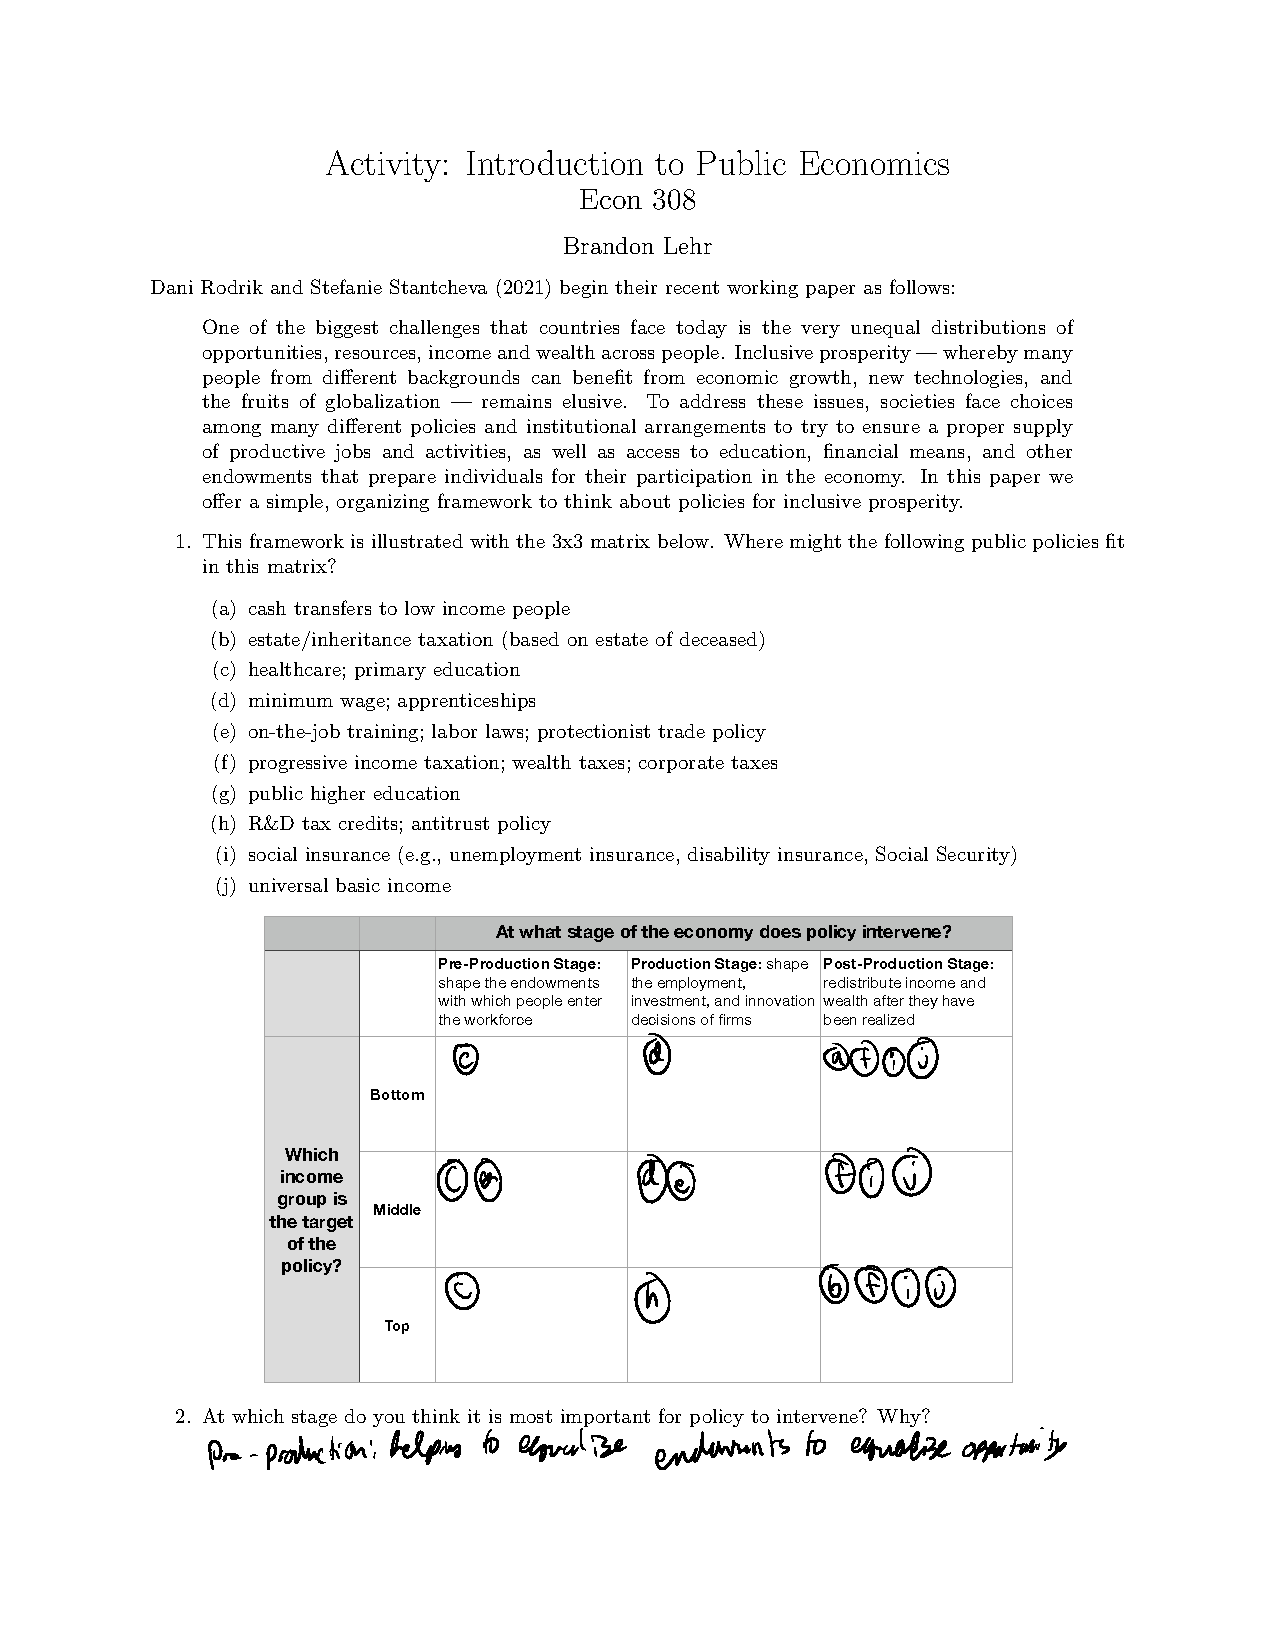
\includegraphics[width=\textwidth]{Activity_1.pdf}
      \end{center}
    \end{problem}
  \end{problem}
  \begin{problem}{Microeconomic Foundations: Consumer Theory}
    \begin{description}
      \item[Utility function] $u(X,Y)$ translates consumption quantities into utility.
      \item[Indifference curve] A graphical representation of all bundles of goods that make an individual equally well off. Mathematically, an indifference curve is the set of all bundles $(X,Y)$ such that $u(X,Y) = U$ for some utility level $U$.
      \item[Marginal Rate of Substitution] $MRS_{XY}$ is the negative slope of the indifference curve --- it's the rate at which the consumer will trade $Y$ for $X$.
        \[
          MRS_{XY} = \frac{\partial u/\partial X}{\partial u/\partial Y}
        \] 
      \item[Budget Constraint] the set of all bundles for which the total amount spent equals income
        \begin{itemize}
          \item Let $I$ indicate income and $P_X$ and $P_Y$ represent the prices of goods $X$ and $Y$ respectively.
          \item The budget constraint is the line segment $P_X X + P_Y Y = I$.
          \item The slope of the budget constraint is $-\frac{P_X}{P_Y}$.
        \end{itemize}
      \item[Utility Maximization] A rational consumer maximizes utility subject to the budget constraint via the parallel conditions of tangency ($MRS_{XY} = \frac{P_X}{P_Y}$) and the budget constraint ($P_X X + P_Y Y = I$).
      \item[Demand Functions] Utility maximization generates demand functions (quantity in terms of price) $X(P_X,P_Y,I)$ and $Y(P_X,P_Y,I)$. There are two primary canonical utility functions.
        \begin{itemize}
          \item Cobb-Douglas: $u(X,Y) = A\ln(X) + B\ln(Y)$, or $u(X,Y) = X^A \cdot Y^B$. The demand function for this utility function yields that $P_X$ has no effect on $Y$ and $P_Y$ has no effect on $X$.
          \item Quasilinear: $u(X,Y) = v(X) + BY$ where $v'(X)>0>v''(X)$ (i.e., concave down, sloping up). The demand function for this utility function yields that $I$ has no effect on $X$ assuming an interior solution.
        \end{itemize}
      \item[Price Effects] The impact of a change in $P_X$ on demand for $X$ is composed into two effects:
        \begin{itemize}
          \item Substitution Effect: change in consumption due to the change in relative prices, with utility held equal. When the price of a good increases, the substitution effect is always negative, and vice versa.
          \item Income Effect: change in consumption due to a change in purchasing power as a result of the price change, where relative prices are held constant at the final price ratio. Income effects can be positive or negative depending on the type of good.
          \item The total effect is equal to the income effect and the substitution effect.
        \end{itemize}
    \end{description}
    \begin{center}
      \begin{tcbraster}[raster columns = 1,colframe = black!75!white,colback=white,title=Income and Substitution Effects]
        \tcbincludepdf[width=10cm]{images/income_substitution.pdf}
      \end{tcbraster}
    \end{center}
    \begin{description}
      \item[Price Elasticity] The price elasticity of demand is the \% change in demand caused by a 1\% change in price of a good.
        \[
          E^D = \frac{dD}{dP}\frac{P}{D}
        \] 
      Elasticities are \textit{unit-free}, typically negative, and tend not to be constant along a demand curve.
    \end{description}
  \end{problem}
  \begin{problem}{Game Theory}
    Some decision problems involve strategic interactions between individuals.
    \begin{itemize}
      \item For example, Antonia and Bruno might care about giving to a local charity, and give $G_A$ and $G_B$ respectively. 
      \item Their utility functions depend on each other $u_A(G_A,G_B),u_B(G_A,G_B)$.
      \item The \textbf{Nash Equilibrium} yields each individual choosing an action that maximizes their utility \textit{given the other person's behavior}.
    \end{itemize}
  \end{problem}
  \begin{problem}{Social Welfare}
    Economists incorporate distributional concerns by use of social welfare functions.
    \[
      SWF = f(U_1,U_2,\dots,U_n)
    \] 
    We have two canonical social welfare functions:
    \begin{itemize}
      \item Utilitarian SWF: $SWF = U_1 + U_2 + \cdots U_n$.
      \begin{itemize}
        \item Marginal utility decreasing in income $\rightarrow$ redistribution from the rich to the poor.
        \item Taking \$1 from a rich person decreases their utility by a small amount, but transferring to a poor person increases their utility by a large amount.
      \end{itemize}
      \item Rawlsian SWF: $SWF = \min\{U_1,U_2,\dots,U_N\}$
      \begin{itemize}
        \item Social welfare is maximized by maximizing the well-being of the worst-off person.
        \item Rawlsian social welfare is more redistributive than utilitarian social welfare.
      \end{itemize}
    \end{itemize}
    There are a few other philosophies regarding the fairness of economic distribution in society.
    \begin{description}
      \item[Just deserts] Individuals should be compensated in line with their contributions.
      \item[Commodity egalitarianism] Society should ensure that individuals meet a set of basic needs, but beyond that point income distribution is irrelevant.
      \item[Equality of opportunity] Society should ensure that all individuals have equal opportunities for success.
    \end{description}
  \end{problem}
  \begin{problem}{Present Discounted Value}
    The present discounted value of a future value of money $F$ that is received and spent in $n$ periods is:
    \[
      PDV = \frac{F}{(1+r)^n}
    \] 
    For the \textbf{discount rate} $r$, typically the interest rate.\\

    For a stream of future expenses $F_i$, we use the following formula:
    \[
      PDV = \sum_{i = 1}^{n} \frac{F_i}{(1+r)^i}
    \] 
    If the values of $F_i$ are equal, then $PDV = \frac{F}{r}$, via the geometric series formula.
  \end{problem}
  \begin{problem}{Activity 2}
   \begin{tcbraster}[raster columns = 1,colframe = black!75!white,colback=white]
     \tcbincludepdf{images/Activity_2.pdf}
   \end{tcbraster} 
  \end{problem}
  \begin{problem}{Empirical Tools of Public Economics}
    \textbf{Identification Problem}: When two variables, $A$ and $B$, are correlated with each other, how do you identify which is causing which (or if both are being caused by something else)? Could the correlation be spurious?
    \begin{problem}{Spurious Correlation}
      \begin{tcbraster}[raster columns = 1,colframe = black!75!white,colback=white]
        \tcbincludepdf{images/spurious_correlation.pdf}
      \end{tcbraster}
    \end{problem}
    \begin{problem}{Randomized Controlled Trials}
      The gold standard of experimentation.
      \begin{itemize}
        \item One group obtains the treatment, one gets the placebo.
        \item The two groups must have close to identical traits aside from the treatment, which is part of the ``control.''
      \end{itemize}
      Randomized controlled trails tend to be common in science, and have grown in popularity in the social sciences, but for economics, RCTs are often difficult to carry out (after all, you cannot split up the timeline).
      \begin{problem}{Limitations of RCTs}
        External validity: it's difficult to apply the outcomes of a randomized controlled trial to other contexts.\\

        Attrition: unequal loss of participants (i.e., people in the control group drop out more than the treatment group, or vice versa).\\

        Unethicality: little feedback on the part of participants, and the interests of participants aren't necessarily taken into account.
      \end{problem}
    \end{problem}
    \begin{problem}{Observational Data}
      Data generated by individual behavior observed in the real world, not in specially-designed experiments.
      \begin{itemize}
        \item Time Series analysis: changes in two different stats over time and trying to find results from said changes.
        \item Cross-Sectional Regression Analysis: finding a relationship between two variables with many data samples.
          \[
            Y_i = \alpha + \beta X_i + \epsilon_i
          \] 
          The OLS estimate, $\hat{\beta}$, is the slope of the data. In order for this relationship to be causal, the error term, $\epsilon_i$, must be uncorrelated with $X_i$.
      \end{itemize}
    \end{problem}
    \begin{problem}{Quasi-Experiments}
      Changes in the economic environments that create nearly identical treatment and control groups for studying the effect of that environmental change, allowing economists to take advantage of quasi-randomization created by external forces.
    \end{problem}
  \end{problem}
  \begin{problem}{Activity 3}
   \begin{tcbraster}[raster columns = 1,colframe = black!75!white,colback=white]
     \tcbincludepdf{images/Activity_3.pdf}
   \end{tcbraster}
  \end{problem}
  \begin{problem}{Market Failures: Externalities}
    The most classic market failure is \textit{externalities}: when the fully private costs/benefits and the social costs/benefit are misaligned. For example, possibly the most important example of a \textit{negative} externality is climate change from CO$_2$ emissions, a byproduct of industrial development.\\

    Economists focus on balancing the total costs (private + social) of pollution with the total benefits (private + social) from pollution.
    \begin{center}
      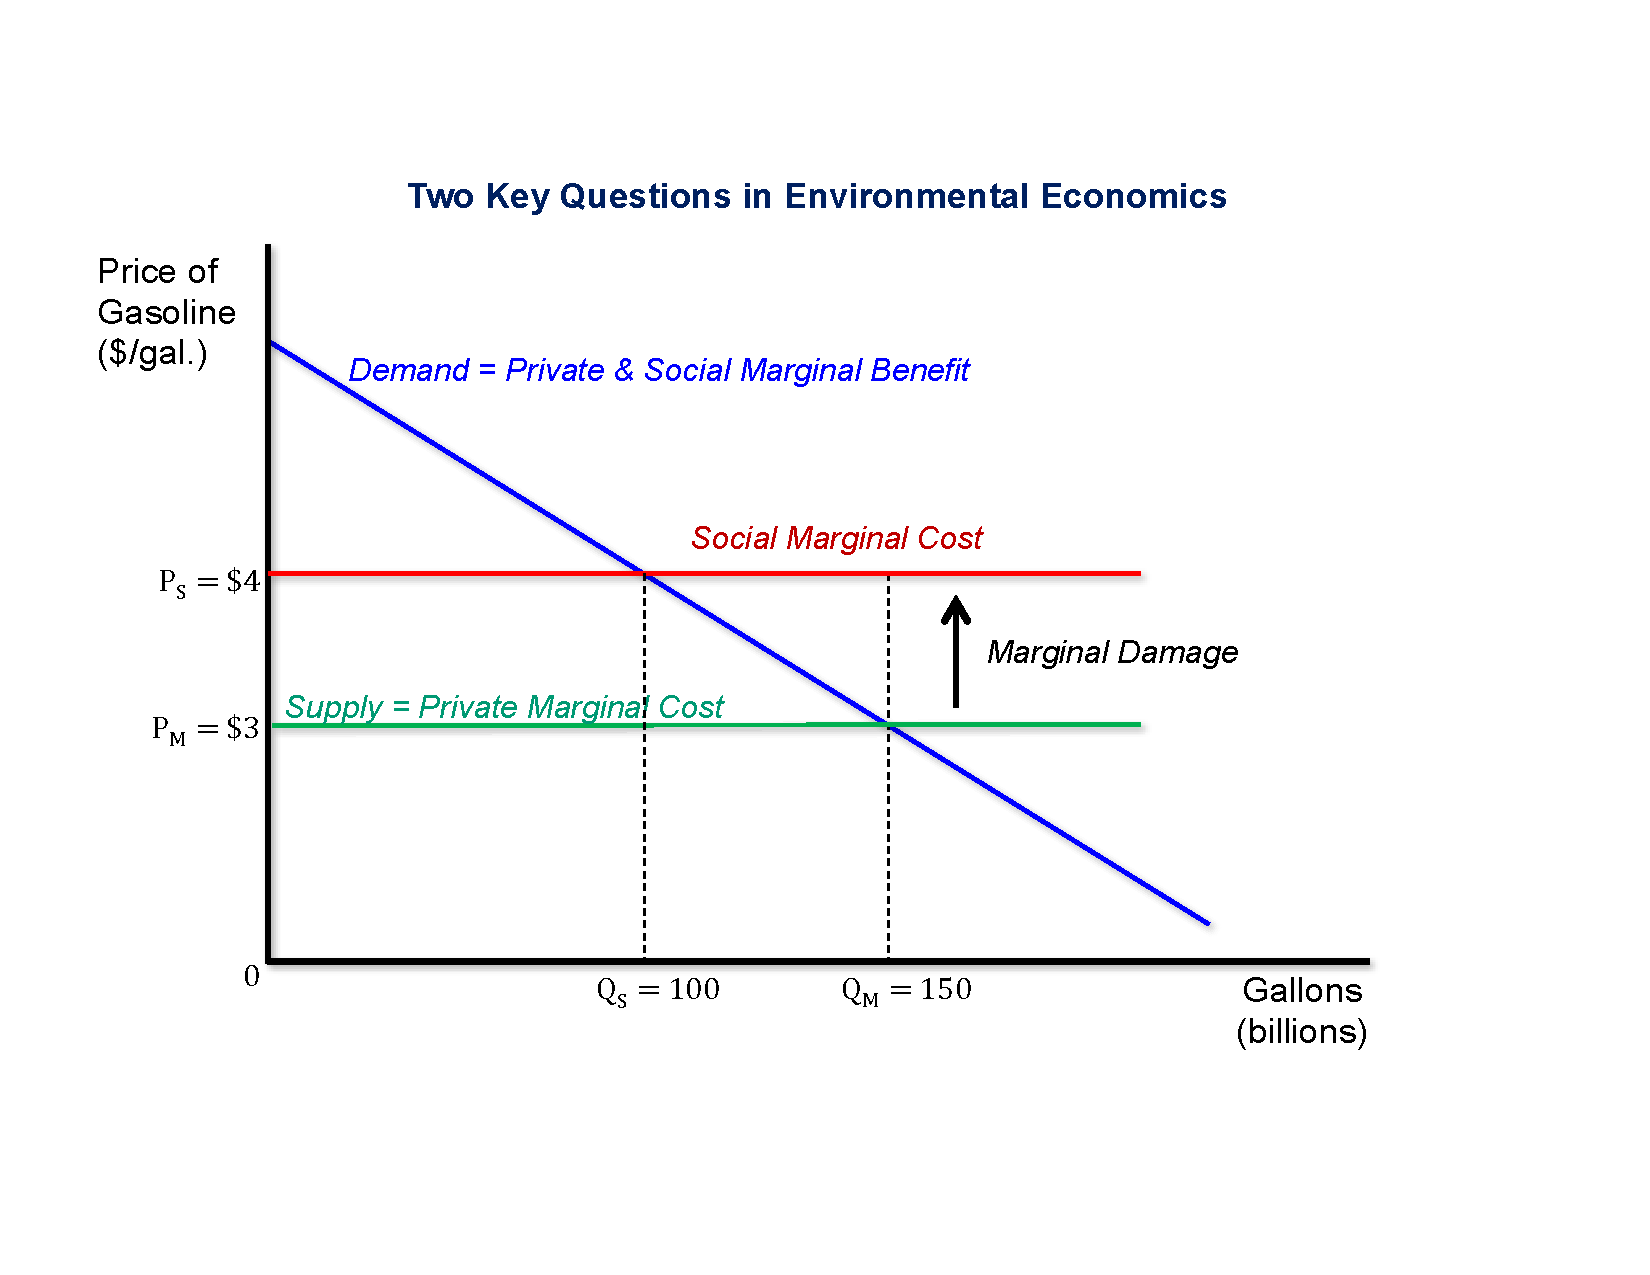
\includegraphics[width=\textwidth]{climate_change_externalities.pdf}
    \end{center}
    The top triangle represents the deadweight loss because the problem of underpriced externalities is one of \textit{overproduction}, not of underproduction. We are facing two questions:
    \begin{itemize}
      \item How do we calculate the marginal social cost of pollution?
      \item What is the best way to reach the marginal social cost of pollution?
    \end{itemize}
    \begin{problem}{Estimating the social cost of carbon}
      \begin{description}
        \item[Step 1:] How does one extra ton of CO$_2$ impact the climate?
        \item[Step 2:] How does a marginal change in climate affect various human outcomes?
        \item[Step 3:] Calculate the current social cost by converting future costs into current dollars via discounting.
      \end{description}
      For Step 2, economists control for the particular location, and do comparisons over time, and check the average effect across all the locations.\\

      After calculating or estimating future costs, economists need to discount these costs toward the present value.
      \[
        PDV = \frac{C_1}{1+r} + \frac{C_2}{(1+r)^2} + \cdots
      \] 
      where $r$ is the \textit{social discount rate}, the rate at which society is willing to trade off between consumption today and consumption tomorrow.\\

      Changes in $r$ matter a lot:
      \begin{itemize}
        \item If $r$ is large (i.e., we don't care much about future generations), then carbon costs are not large.
        \item If $r = 0$ (i.e., we care equally about all generations), then carbon costs can be infinite.
      \end{itemize}
      Various economists calculated different social discount rates:
      \begin{itemize}
        \item Giglio, Maggiori, and Stroebel calculated $2.6\%$, by using differences in price between perpetual ownership and 100 year leases.
        \item The Obama administration used a 3\% discount rate, implying the social cost of carbon was \$42/ton.
        \item The Trump administration used a 7\% discount rate, implying the social cost of carbon was \$5/ton
        \item The Biden administration uses an estimate of \$51/ton.
      \end{itemize}
    \end{problem}
  \end{problem}
  \begin{problem}{Policy Solutions}
    We can use \textit{pigouvian taxes} to force market participants to internalize the cost of the externality.\\

    Alternatively, we can use \textit{industrial policy}, to restructure the market in order to pursue a public goal.
    \begin{itemize}
      \item Subsidizing clean energy.
      \item Research in clean energy technologies both public and private.
      \item Phase out carbon in various economic sectors and weaken fossil fuels.
    \end{itemize}
    We have seen great dividends so far: solar and wind have become extremely cheap to produce, and replacing coal with natural gas has yielded emissions reductions that were greater than targets. The Biden administration focused on making clean energy even cheaper via the Inflation Reduction Act.
  \end{problem}
  \begin{problem}{Activity 4}
    \begin{tcbraster}[raster columns = 1,colframe = black!75!white,colback=white]
      \tcbincludepdf{images/Activity_4.pdf}
    \end{tcbraster}
  \end{problem}
  \begin{problem}{Public Goods}
    A public good is not something that's merely good for the public, but it is specifically a good that is rival and non-excludable (essentially, the same quantity of the good has to be available to every person.)\\

    The optimal level of publi goods is when the \textit{vertical} sum of individual demand curves equals the marginal cost of providing the public good. The reason the demand curves are added vertically is because market participants can share the public goods.\\

    Recall that $MRS_{GX}$ of a public good $G$ for a private good $X$ is how much an individual values an additional unit of $G$ in terms of unit of $X$.
    \begin{align*}
      MRS_{GX} &= \frac{MU_G}{MU_X}
    \end{align*}
    The total number of units of $X$ society is willing to give up for $1$ more unit of $G$ is the sum of all $MRS_{GX}$.\\

    Assuming that $P_X = 1$, this is a measure of how many dollars society is willing to pay for $1$ more unit of $G$. The societal value is the sum of the different $MRS_{GX}$ values:
    \begin{align*}
      MC_G &= \sum_{I=1}^{N} MRS_{GX}^I
    \end{align*}
    This is the \textit{Samuelson Rule}.
  \end{problem}
  \begin{problem}{Private Provision of Public Goods}
    \begin{itemize}
      \item The private outcome is the Nash equilibrium of a game where individuals choose how to allocate income between $G$ and $X$, taking into account spending on $G$ by others.
      \item The Nash equilibrium does not satisfy the Samuelson Rule.
      \item Public goods problems can be described as \textbf{free-rider} problems (i.e., underproduction).
      \item There is not necessarily zero private provision of public goods. Private provision works well in the following cases:
        \begin{itemize}
          \item Some people have much higher marginal rate of substitution (i.e., they care more than others).
          \item Altruism: people care purely about giving to others.
          \item Warm Glow: people get utility from giving to others.
        \end{itemize}
    \end{itemize}
    There is experimental evidence of free-riding; for example, Marwell and Ames (1981) had an experiment where they tested whether subjects were willing to contribute to a public good, where the Nash equilibrium was that people didn't contribute, and the social optimum was everyone contributing.\\

    People are willing to cooperate at first, but then get upset as time goes on and retaliate.
  \end{problem}
  \begin{problem}{Public Goods Example}
    Let there be $2$ people, with the same utility functions over $X,F$, where $X$ is a private good and $F$ is a public good:
    \begin{align*}
      U_i(X_i,F) &= 2\ln(X_i) + \ln(F)\tag*{for $i=1,2$}
    \end{align*}
    Each participant has a budget constraint, where $P_X$ and $P_F$ are both $1$.
    \begin{align*}
      X_i + F_i = 100\tag*{for $i=1,2$}
    \end{align*}
    Where $F = F_1 + F_2$.
    \begin{description}
      \item[Maximize Person 1's utility:] (i.e., finding the best response function)
    \end{description}
    \begin{align*}
      0 &= \frac{\partial U_1}{\partial F_1}\\
      0 &= -\frac{2}{100-F_1} + \frac{1}{F_1 + F_2}\tag*{recall that $X_1 = 100-F_1$}\\
      2(F_1 + F_2) &= 100-F_1\\
      F_1 &= \frac{100-2F_2}{3}
    \end{align*}
    Since this is a symmetric game, we know that the best response function for Person 2 is $F_2 = \frac{100-2F_1}{3}$.\\

    The Nash equilibrium is when all players are playing their best response to each other. Since the game is symmetric, we know that $F_1^* = F_2^*$
    \begin{align*}
      F_1^* &= \frac{100-2F_1^*}{3}\\
      F_1^* &= 20\\
      F_2^* &= 20
    \end{align*}
    The social optimum (following the Samuelson Rule) is as follows:
    \begin{align*}
      MRS_{FX}^1 + MRS_{FX}^2 &= 1\\
      \frac{MU_F}{MU_{X_1}} + \frac{MU_F}{MU_{X_2}}  &= 1\\
      \frac{1}{2}\frac{X_1}{F} + \frac{1}{2}\frac{X_2}{F} &= 1\\
      2 &= \frac{X_1 + X_2}{F}\\
      F &= \frac{X_1 + X_2}{2}\\
      F &= \frac{200-F}{2}\\
      F &= \frac{200}{3}
    \end{align*}
  \end{problem}
  \begin{problem}{Public Provision of Public Goods}
    The primary problem of public provision of public goods is \textit{crowding out} (i.e., reduced private contributions to public goods). There are two key assumptions of one-to-one private contributions:
    \begin{itemize}
      \item Individuals do \textit{not} have warm glow preferences.
      \item Private actors are contributing to the public good.
    \end{itemize}
    There is empirical evidence of partial crowd-out (i.e., reduction in charitable giving as government spending is increased). However, since people tend to give to charity due to warm glow preferences and social pressures, the crowd-out is not one-to-one. Hungerman (2005) estimates that the crowd-out effect is 20–40 cents per dollar of welfare spending.
  \end{problem}
  \begin{problem}{Activity 5}
    \begin{tcbraster}[raster columns = 1,colframe = black!75!white,colback=white]
      \tcbincludepdf{images/activity_5.pdf}
    \end{tcbraster}
  \end{problem}
  \begin{problem}{Three Questions in Public Economics}
    \begin{description}
      \item[Descriptive:] What are the effects of interventions and policies (empirical)?
      \item[Normative:] What is the optimal policy (theoretical)?
      \item[Public Choice:] Why do governments choose the policies they do (mixture of theory and empirics)?
    \end{description}
  \end{problem}
  \begin{problem}{Rules of Social Decision}
    There are at least 2 individuals with transitive preferences over at least $3$ options. A \textbf{social decision rule} aggregates these preferences into a social preference over these options.\\

    Suppose we want our social decision rule to satisfy the following properties:
    \begin{description}
      \item[Transitive:] if $a$ is ranked above $b$ by our rule, and $b$ is ranked above $c$ by our rule, then $a$ has to be ranked above $c$ by our rule.
      \item[Pareto Efficiency:] if everyone prefers $a$ to $b$, then our rule should rank $a$ above $b$.
      \item[Independence of Irrelevant Alternatives:] the ranking of any two options depends only on how individuals rank the options (and not the ranking of other alternatives).
      \item[Non-dictatorship:] There is no individual whose preference ranking of any two options matches the social ranking (no matter the preferences of others).
    \end{description}
    All of these seem reasonable, so they must be possible, right? Well...
  \end{problem}
  \begin{problem}{Arrow's Impossibility Theorem}
    Arrow's Impossibility Theorem is the following:
    \begin{quote}
        There is no social decision rule that satisfies the properties of Universality (i.e., transitivity), Pareto Efficiency, Independence of Irrelevant Alternatives, and Non-dictatorship.
    \end{quote}
    The implication of Arrow's Impossibility Theorem means that the only voting method that satisfies the first three properties of our social rule is a dictatorship. However, since we don't want a dictatorship, we can use the following:
    \begin{itemize}
      \item Restrict preferences (i.e., transitive is insufficient)
      \item Relax Independence of Irrelevant Alternatives, and let intensity of preferences play a role (for example, the Samuelson rule).
    \end{itemize}
  \end{problem}
  \begin{problem}{Case Study: Majority Voting}
    Pairwise majority voting is a mechanism to aggregate individual votes into a social decision. Since Majority Voting is obviously Pareto efficient and non-dictatorial, and satisfies IIA because the ranking of $a$ over $b$ only depends on how many people vote $a$ vs. how many people vote $b$. Therefore, we must have that majority voting fails transitivity.\\

    Consider an election for funding public schools:
    \begin{problem}{Majority Voting ``Working''}
      \begin{center}
        \renewcommand{\arraystretch}{1.5}
        \begin{tabular}{c|c|c|c|}
          \multicolumn{1}{c}{Preferences} & \multicolumn{3}{c}{Type of Voter}\\
          \cline{2-4}
                                          & Parents ($1/3$) & Elders ($1/3$) & Young Couples ($1/3$)\\
          \cline{2-4}
          First & $H$ & $L$ & $M$\\
          \cline{2-4}
          Second & $M$ & $M$ & $L$\\
          \cline{2-4}
          Third & $L$ & $H$ & $H$\\
          \cline{2-4}
        \end{tabular}
      \end{center}
      \begin{itemize}
        \item $M>_s L$
        \item $L >_s H$
        \item $M >_s H$
      \end{itemize}
      Therefore, $M>L>H$, and so $M$ is the social choice made by pairwise majority voting.
    \end{problem}
    \begin{problem}{Majority Voting ``Failing''}
      \begin{center}
        \renewcommand{\arraystretch}{1.5}
        \begin{tabular}{c|c|c|c|}
          \multicolumn{1}{c}{Preferences} & \multicolumn{3}{c}{Type of Voter}\\
          \cline{2-4}
                                          & Public School ($1/3$) & Private School ($1/3$) & Young Couples ($1/3$)\\
          \cline{2-4}
          First & $H$ & $L$ & $M$\\
          \cline{2-4}
          Second & $M$ & $H$ & $L$\\
          \cline{2-4}
          Third & $L$ & $M$ & $H$\\
          \cline{2-4}
        \end{tabular}
      \end{center}
      \begin{itemize}
        \item $M >_s L$
        \item $L >_s H$
        \item $H >_s M$
      \end{itemize}
      We are now stuck in a cycle $M>L>H>M>\cdots$. This election fails to successfully aggregate the preferences of the populace.
    \end{problem}
    A way to get out of the trap of transitivity is to rule out preferences that are not single-peaked (i.e., one local maximum).\\

    However, when we have single-peaked preferences, we have that the preferences of the median voter is that which is preferred by society.
  \end{problem}
  \begin{problem}{Implications of the Median Voter Theorem}
    If we restrict our analysis to single-peaked preferences, majority voting is a social decision rule that satisfies all desirable properties.\\

    However, this means majority voting does not imply efficiency. For example, if a public good is efficient, but because a minority has a large marginal benefit and the majority has a small marginal benefit, the public good will get rejected. What matters for efficiency is the \textit{average} marginal benefit across individuals, not the \textit{median} marginal benefit.\\

    However, the median voter theorem doesn't really hold in real life (i.e., Democrats close to the median still vote similar to their caucus, and Republicans close to the median still vote similar to their caucus).
  \end{problem}
  \begin{problem}{Activity 6}
    \begin{tcbraster}[raster columns = 1,colframe = black!75!white,colback=white]
      \tcbincludepdf{images/activity_6.pdf}
    \end{tcbraster}
  \end{problem}
  \begin{problem}{Local Public Goods: the Tiebout Hypothesis}
    Tiebout (1956) asks the following: What is it about the private market that guarantees optimal provision of private goods that is missing in the case of public goods?\\

    Proposed answer: \textbf{shopping} and \textbf{competition}. However, we can see this somewhat resolved in the local level:
    \begin{itemize}
      \item Individuals can vote with their feet (i.e., move between different cities)
      \item The threat of exit can induce competition in the provision of public goods.
    \end{itemize}
    \begin{quote}
        Just as the consumer may be visualized as walking to a private market place to buy his goods,... we place him in the position of walking to a community where the prices (taxes) of community services are set. Both trips take the consumer to the market. There is no way in which the consumer can avoid revealing his preferences in a spatial economy.
    \end{quote}
  \end{problem}
  \begin{problem}{Modeling the Tiebout Hypothesis}
    Suppose there are $2N$ families, each with identical income $Y$, and 2 towns with $N$ homes each.\\

    Towns $1$ and $2$ supply levels $G_1$ and $G_2$ of local public goods at $MC_G = 1$.
    \begin{itemize}
      \item $N$ families with kids, with $U^K(C,G)$ over private consumption $C$ and public schools $G$.
      \item $N$ elderly families, with $U^E(C)$ over only private consumption $C$.
    \end{itemize}
    The allocation of families across towns is a \textbf{Tiebout Equilibrium} if and only if:
    \begin{enumerate}[(1)]
      \item No two families want to exchange locations across towns; and
      \item In each town, $G$ is decided by the median voter and financed \textit{equally} by town residents.
    \end{enumerate}
    \begin{description}
      \item[Family Budget Constraint:] $Y = C + G/N$, where $P_C = 1$ and $P_G = 1/N$
        \begin{itemize}
          \item If the majority in the town is elderly, then $G = 0$, as that maximizes $U^E(Y-G/N)$. 
          \item If the majority in the town is families with kids, then $G^*$ is that which maximizes $U^K(Y-G/N,G)$ such that $MRS_{GC}^K = \frac{1}{N}$.
        \end{itemize}
    \end{description}
    \begin{problem}{Tiebout Theorem}
      \begin{description}
        \item[Part 1 (Sorting):] In equilibrium, families will sort themselves in towns according to their taste for the public good (1 town with elderly only, one town with families with kids).
        \item[Part 2 (Efficiency):] In each town, the level of local public good is efficient.
          \begin{itemize}
            \item In the elderly town, $G = 0$, which is efficient as nobody values $G$.
            \item In the kids town, $\sum MRS_{GC}^{K} = \frac{1}{N} = 1 = MC_G$, which is the Samuelson Rule for efficiency in public goods provision.
          \end{itemize}
      \end{description}
    \end{problem}
    A Tiebout equilibrium may not be socially desirable if there is a public interest in integration within towns and for reducing social distance across groups (i.e., intergroup contact theory).
  \end{problem}
  \begin{problem}{Assumptions of the Tiebout Hypothesis}
    \begin{enumerate}[(1)]
      \item High Mobility: may be impeded by (artificial or natural) barriers to entry, preferences over other qualities.
      \item Perfect information: lack of knowledge about the quality of public goods.
      \item Scale: inability to fund public goods for one's preferences.
      \item Variety: enough options of types of towns.
      \item No externalities or spillovers: otherwise, public good will be underproduced.
      \item Equal financing of the public good (poll tax): local public finance generally tends to be based on property or sales tax.
    \end{enumerate}
  \end{problem}
  \begin{problem}{Financing Local Public Goods}
    \begin{itemize}
      \item Towns finance their local public goods through property taxation, where the rich pay more than the poor.
      \item Property taxes induce the poor to chase the rich, while the rich want to segregate themselves from the poor.
      \item The rich tend to implement mechanisms to prevent free-riding: making houses expensive.
        \begin{itemize}
          \item Zoning laws restrict supply of housing.
        \end{itemize}
      \item Discriminatory practices (such as deed restrictions) to stop poorer people from living near rich people.
    \end{itemize}
  \end{problem}
  \begin{problem}{Tiebout Implications for Redistribution}
    It's very hard for a local government to redistribute from the rich to the poor (easy exit).\\

    In localities, to avoid migration, public goods financing needs to have strong \textbf{tax-benefit linkages} (i.e., the relationship between taxes and the government benefits need to be very explicit and visual).\\

    Higher levels of government can redistribute across communities using taxes to directly or indirectly incentivize public goods spending.\\

    For example, state governments can match, in which case the price of public goods goes from $1$ to  $\frac{1}{1+m}$, for $m$ being the value of the match. However, with any intergovernmental transfers (either matching or intergovernmental transfer), there is a potential for crowd-out.
  \end{problem}
  \begin{problem}{Flypaper Effect}
    Empirical evidence suggests that the crowd-out of state spending by federal spending is low and often close to zero --- ``the money sticks where it lands.''\\

    More recent studies show that while there is a flypaper effect in the short run, there is substantial crowd-out from block grants in the long run.
  \end{problem}
  \begin{problem}{Activity 7}
    \begin{tcbraster}[raster columns = 1,colframe = black!75!white,colback=white]
      \tcbincludepdf{images/activity_7.pdf}
    \end{tcbraster}
  \end{problem}
  \begin{problem}{Education: Motivations for Government Intervention}
    Education is one of the largest public goods provided by the government: 6\% of GDP and 12.7\% of total government expenditure.\\

    However, education is not a pure public good:
    \begin{itemize}
      \item Excludable: private education that charges money, or only allow a particular enrollment area.
      \item Rival: there are a limited number of seats in a school (capacity constraints, quality degrades if there are too many students).
      \item Private returns: your investment in education primarily benefits you.
    \end{itemize}
    So, why should the government be involved?
    \begin{itemize}
      \item Positive Externalities: a more educated workforce might lead to more productivity and technology.
      \item Family Failures: if the parental units are unable to provide for education that the child desires, the government involvement is welfare-improving.
      \item Borrowing constraints: education can be very expensive, and loans are less available (no collateral).
      \item Behavioral Mistakes: maybe you don't know what's in your best interest.
    \end{itemize}
  \end{problem}
  \begin{problem}{Education Reform}
    \begin{description}
      \item[Supply-Side:] Improving the process of education:
        \begin{itemize}
          \item Smaller classes
          \item Improving teachers
          \item Charter Schools
        \end{itemize}
      \item[Demand-Side:] Improving individual funding:
        \begin{itemize}
          \item Vouchers
          \item Subsidies/Loans/Grants
        \end{itemize}
    \end{description}
    \begin{problem}{Class Size}
      We cannot simply compare outcomes for students in small vs. large classes because of omitted variables (like income/family education).\\

      In Sweden, class size cuts off at 30 students --- this yields quasi-experimental variation, which we can use to see causality. Frederiksson, Ockert, and Oosterbeek (2013) found that there was a 4\% jump in wages for students in a smaller class.
    \end{problem}
    \begin{problem}{Teacher Quality}
      One measure of teacher quality: teacher value-added or test score-based metrics of teacher performance.
      \begin{itemize}
        \item How much does a teacher raise their students' test scores on average (adjusting for noise and controlling for differences in students)?
      \end{itemize}
      How do we measure the impact of teacher quality?
      \begin{itemize}
        \item The ideal RCT randomizes students to teachers with different levels of value-added.
        \item Quasi-Experiment: use the turnover in teachers across school years.
      \end{itemize}
      Chetty, Friedman, and Rockoff (2014) use data on all kids who went to NYC public schools in 1989 and link to tax records.\\

      They found an increase of 1.5\% in earnings and 1.5\% reduction in teenage births going from a 5th percentile teacher to a 95th percentile teacher.\\

      Most school districts do not use any performance measures to evaluate teachers.
    \end{problem}
    \begin{problem}{Charter Schools}
      Charter schools are schools financed with public funds that are not usually under the direct supervision of local school boards or subject to state regulation.\\

      To measure effectiveness, one cannot simply compare outcomes at charters with public schools due to different types of students.\\

      Quasi-experiment: compare charter lottery winners with charter lottery losers (for schools that use a lottery).\\

      In Massachusetts, Angrist, Pathak, and Walters (2013) found that urban charter schools boost achievement while non-urban charters reduce achievement.\\

      Charters tend to constitute a market-based approach to education, but there are some limitations:
      \begin{itemize}
        \item Demand-side limitations: Families may not have enough information to choose the best charter schools for their children.
        \item Supply-side limitations: Schools have an incentive to reject less-qualified applicants (nicknamed ``cream-skimming'').
      \end{itemize}
    \end{problem}
    \begin{problem}{Vouchers}
      With free public education, there is an incentive to \textit{cluster} their total education spend around where the public school's funding is. However, if the money for public education is given equally to all families, it's akin to a conditional block grant.\\

      Vouchers are meant to induce every household to increase their spending on education.\\

      However, there are mixed results from using vouchers:
      \begin{itemize}
        \item Angrist et al. (2002), using lottery assignment of vouchers in Colombia, show positive effects on education.
        \item Abdulkadiroglu, Pathak, and Walters (2018) used randomized lotteries to evaluate the Louisiana Scholarship program, and found lower achievement by those who win vouchers compared to those who did not.
      \end{itemize}
    \end{problem}
  \end{problem}
  \begin{problem}{Government Involvement in Higher Education}
    \begin{itemize}
      \item State Provision (about \$82 billion)
      \item Pell Grants (\$22.4 billion)
      \item Direct Student Loans (\$34.4 billion)
      \item Other reliefs (\$10.3 billion)
    \end{itemize}
    Supply trends:
    \begin{itemize}
      \item Priate non-profit universities have inelastic supply (fixed student bodies).
      \item Historically, supply for higher education has been administered by public universities (creating new UCs/Cal States/etc.)
      \item Supply has been provided by for-profit schools, although for-profit schools tend to provide little in benefits to students.
    \end{itemize}
    Reduced (direct) state funding has led to higher tuition and student debt.\\

    Additionally, women have been earning many more higher education degrees than men.\\
    \begin{problem}{Effect of Higher Education on Mobility}
      Chetty et al. (2017) study parental income and student earning outcomes by college.\\

      Certain schools (Harvard and Berkeley) tend to have high quantities of students in the top 20\% of the income distribution, while others like SUNY-Stony Brook tend to have more equal student populations.\\

      They found that education tends to have a flattening effect (i.e., poor kids and rich kids tend to have more similar outcomes when educated).\\

      The mobility rate for a given school can be found by (i.e., the rate of children born in the bottom quintile ending up in the top quintile) can be calculated by finding the success rate (probability that a child moves from the bottom quintile to the top quintile) and multiplying by the proportion of parents in the bottom quintile.\\

      The top college by mobility rate was Cal State LA, and the top ten tended to be open-access public universities (i.e., Glendale Community College, City University of New York, etc.).
    \end{problem}
  \end{problem}
\end{document}
